
To construct effective metaheuristics without constraining the solver to a predefined top-level architecture, we adopt a bottom-up automatic algorithm design (AAD) paradigm.
Unlike top-down approaches that select among a few rigid, monolithic algorithm templates, the bottom-up approach focuses on designing modular, fine-grained algorithmic components.
Automated configurators then combine these low-level building blocks to assemble novel and hybrid metaheuristic architectures automatically \citep{de2018automatic}.
We selected these algorithmic building blocks primarily from the existing JITJSS literature, while also incorporating effective strategies from related scheduling domains.

To specify valid combinations of algorithmic components systematically, we formalize the design space using a context-free grammar in Backus-Naur Form (BNF) \citep{mascia2013grammars}, shown in Figure~\ref{fig:grammar}.
In our BNF grammar, every derivation from the start symbol \texttt{<algorithm>} produces a syntactically valid algorithm.
Non-terminal symbols represent design decisions, such as initial solution generation (\texttt{<initial\_sol>}), neighborhood selection (\texttt{<neighborhood>}), search procedures (\texttt{<search>}), and sequence schedulers (\texttt{<scheduler>}), while terminal symbols represent specific algorithmic operators or numerical parameters.

Following the methodology proposed by \citet{mascia2013grammars} and \citet{mascia2014grammar}, we map non-terminal symbols directly to categorical, ordinal, or numerical parameters within an Automatic Algorithm Configuration (AAC) framework.
Deriving a non-terminal symbol from another non-terminal symbol creates conditional parameter relationships within the configurator, ensuring that the tool evaluates parameters only when the corresponding algorithmic component is active.
To accommodate recursive search structures, such as nested local searches or iterated metaheuristics, within a finite parameter space, we follow \citet{mascia2013grammars} by duplicating parameter blocks for each allowed recursion level $i$, making level $i+1$ parameters conditional on the recursive choice at level $i$.

\begin{figure}[t]
\centering
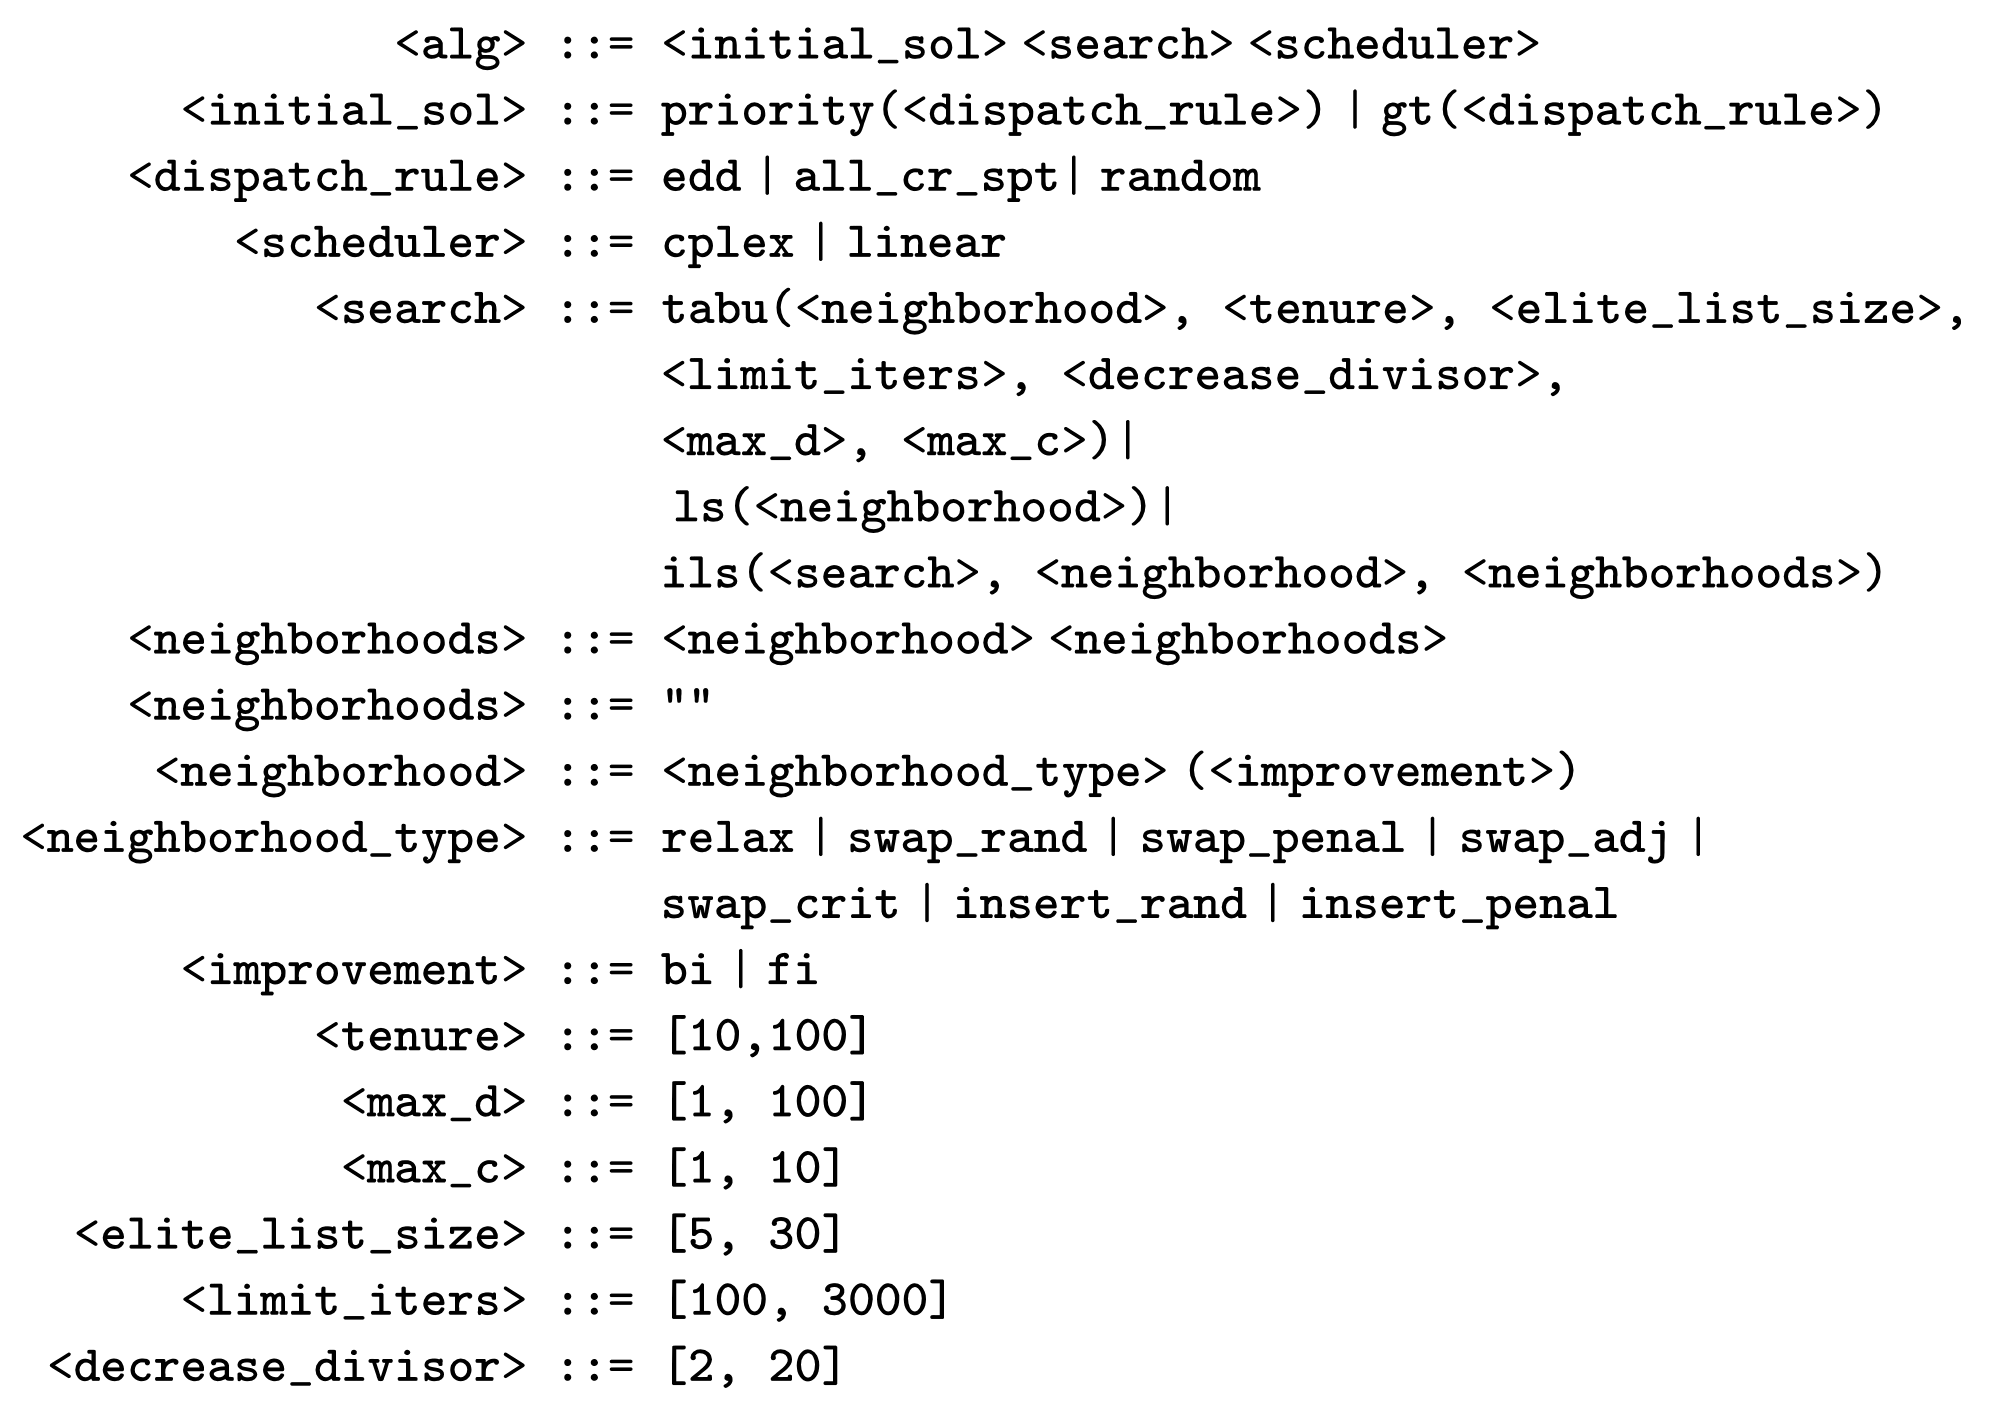
\includegraphics[width=1\linewidth]{img/grammar.png}
\caption{Context-free grammar in Backus-Naur Form (BNF) defining the JITJSS algorithmic design space.}
\label{fig:grammar}
\end{figure}

\subsection{Initialization Rules }
\label{subsec:initialization_rules}

Initial solution sequences are generated via the non-terminal symbol \texttt{<initial\_sol>}, which selects one of two constructive procedures combined with one priority dispatching rule (\texttt{<dispatch\_rule>}) among Earliest Due Date (\texttt{edd}), random selection (\texttt{random}), and the ALL+CR+SPT (\texttt{all\_cr\_spt}) rule proposed by \citet{wang2014variable}.
The first constructive option is a standard dispatching procedure (\texttt{priority}) that iteratively selects the next operation to schedule directly from a candidate list by evaluating the chosen priority rule.

The second option is the Giffler--Thompson (GT) method \citep{giffler1960algorithms}, which also employs a chosen dispatching rule, but performs internal filtering operations on the candidate list prior to rule evaluation to guarantee the generation of active schedules without unnecessary machine idle time.
The GT algorithm is included as it serves as the standard constructive procedure across leading JITJSS studies \citep{ahmadian2021meta, abderrazzak2022adaptive, sabri2023reinforcement}.

\subsection{Neighborhood Operators} 
\label{subsec:neighborhood_operators}

\subsection{Search procedures}
\label{subsec:search_procedures}

\subsection{Perturbation Mechanisms }
\label{subsec:perturbation}

\subsection{Exact Timing Sub-Solvers}
\label{subsec:exact_subsolvers}
